\section{Dataset}
\label{sec:dataset}
To train and evaluate our approach we use the public available OuluVS2 database.
The recorded environment used is illustrated in figure \ref{fig:ouluMultiView}, where the multi-view setting can be seen.
The setup make use of five cameras located at different angels in relation to the subject.
For each recorded subject three different scenarios is performed, namely the pronunciation of: 
(1) a sequence of ten fixed digit sequences,
(2) ten daily-use short English phrases and
(3) five randomly selected TIMIT sentences.
Examples of each of these can be seen in table \ref{tab:ouluSecnarioExamp}
A total of 52 different test subject is used, where each subject is pronouncing each phrase three times.

A preprocessed version is available where the recording from different angles is synchronized and the region of interest (ROI) is both segmented, with the recording of interest, and cropped to only contain the mouth region.
An example of the preprocessed data can be seen in figure \ref{fig:ouluPreprocessed}.

\begin{figure}
    \centering
    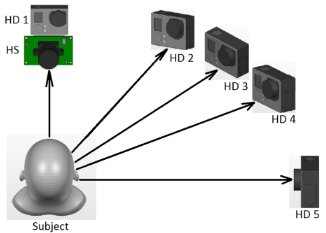
\includegraphics[width=0.6\columnwidth]{fig/ouluMultiView.jpg}
    \caption{Illustration of the multi-view setup used in the OuluVS2 recording}
    \label{fig:ouluMultiView}
\end{figure}
\begin{figure}
    \centering
    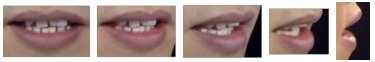
\includegraphics[width=\columnwidth]{fig/ouluPreprocessed.jpg}
    \caption{Example of the preprocessed data with with the region of interest.}
    \label{fig:ouluPreprocessed}
\end{figure}

\begin{table}
    \begin{tabular}{l|p{6.2cm}}
        \multirow{2}{*}{(1) Digits}  
        & "1 7 3 5 1 6 2 6 6 7"\\
        & "4 0 2 9 1 8 5 9 0 4"\\
        \hline
        \multirow{2}{*}{(2) Phrases}  
        & "Thank you"\\
        & "Have a good time"\\
        \hline
        (3) TIMIT & "Chocolate and roses never fail as a romantic gift"
    \end{tabular}
    \caption{Examples of the three different scenarios used}
    \label{tab:ouluSecnarioExamp}
\end{table}
